\documentclass{homework}
\author{Chaklam Silpasuwanchai, Akraradet Sinsamersuk}
\class{AT82.03: Machine Learning}
\title{A1: Predicting Car Price}
\address{}

\graphicspath{{./media/}}
\usepackage{listings}
\usepackage{xcolor}
\definecolor{codegreen}{rgb}{0,0.6,0}
\definecolor{codegray}{rgb}{0.5,0.5,0.5}
\definecolor{codepurple}{rgb}{0.58,0,0.82}
\definecolor{backcolour}{rgb}{0.95,0.95,0.92}

\lstdefinestyle{mystyle}{
    language=Python,
    backgroundcolor=\color{backcolour},   
    commentstyle=\color{codegreen},
    keywordstyle=\color{magenta},
    numberstyle=\tiny\color{codegray},
    stringstyle=\color{codepurple},
    basicstyle=\ttfamily\footnotesize,
    breakatwhitespace=false,         
    captionpos=b,                    
    keepspaces=true,                 
    numbers=left,                    
    numbersep=5pt,                  
    showspaces=false,                
    showstringspaces=false,
    showtabs=false,                  
    tabsize=2
}

\lstset{style=mystyle}


\begin{document} \maketitle

In this assignment, you will solve a problem, i.e., Chaky company makes some car but he has difficulty setting the price for the car.  Please make a simple web-based car price prediction system.

\vspace{0.01\textheight}

\textbf{Note}:  You are ENCOURAGED to work with your friends, but DISCOURAGED to blindly copy other's work.  Both parties will be given 0.

\textbf{Note}:  Comments should be provided sufficiently so we know you understand.  Failure to do so can raise suspicion of possible copying/plagiarism.

\textbf{Note}:  You will be graded upon (1) documentation, (2) experiment, (3) implementation.

\textbf{Note}:  This is a two-weeks assignment, but start early.

\textbf{Deliverables}: The GitHub link containing the jupyter notebook, a README.md of the github, and the folder of your web application called `app'.

\vspace{0.01\textheight}

\hrule

\task \textbf{Preparing the datasets} - Download the \texttt{Car Price} dataset from Google classroom. Perform loading, EDA, preprocessing, model selection, $\cdots$, inference.  Grade will be given based on the how well you adhere to best practices. There are some important coding considerations:

\begin{itemize}
    \item For the feature \texttt{owner}, map \texttt{First owner} to 1, ..., \texttt{Test Drive Car} to 5
    \item For the feature \texttt{fuel}, remove all rows with CNG and LPG because CNG and LPG use a different mileage system i.e., km/kg which is different from kmpl for Diesel and Petrol
    \item For the feature \texttt{mileage}, remove ``kmpl" and convert the column to numerical type (e.g., float).  Hint:  use \texttt{df.mileage.str.split}
    \item For the feature \texttt{engine}, remove ``CC" and convert the column to numerical type (e.g., float)
    \item Do the same for \texttt{max power}
    \item For the feature \texttt{brand}, take only the first word and remove the rest
    \item Drop the feature \texttt{torque}, simply because Chaky's company does not understand well about it
    \item You will found out that \texttt{Test Drive Cars} are ridiculously expensive.  Since we do not want to involve this, we will simply delete all samples related to it.
    \item Since \texttt{selling price} is a big number, it can cause your prediction to be very unstable.  One trick is to first transform the label using \texttt{log transform}, i.e., 
    
    \begin{lstlisting}
        y = np.log(df['selling_price'])
    \end{lstlisting}

    \item During inference/testing, you have to transform your predicted y backed before comparing with \texttt{y test}, i.e., 

    \begin{lstlisting}
        pred_y = np.exp(pred_y)
    \end{lstlisting}
    
\end{itemize}

Your final data should look like this:

\begin{figure}[h]
    \centering
    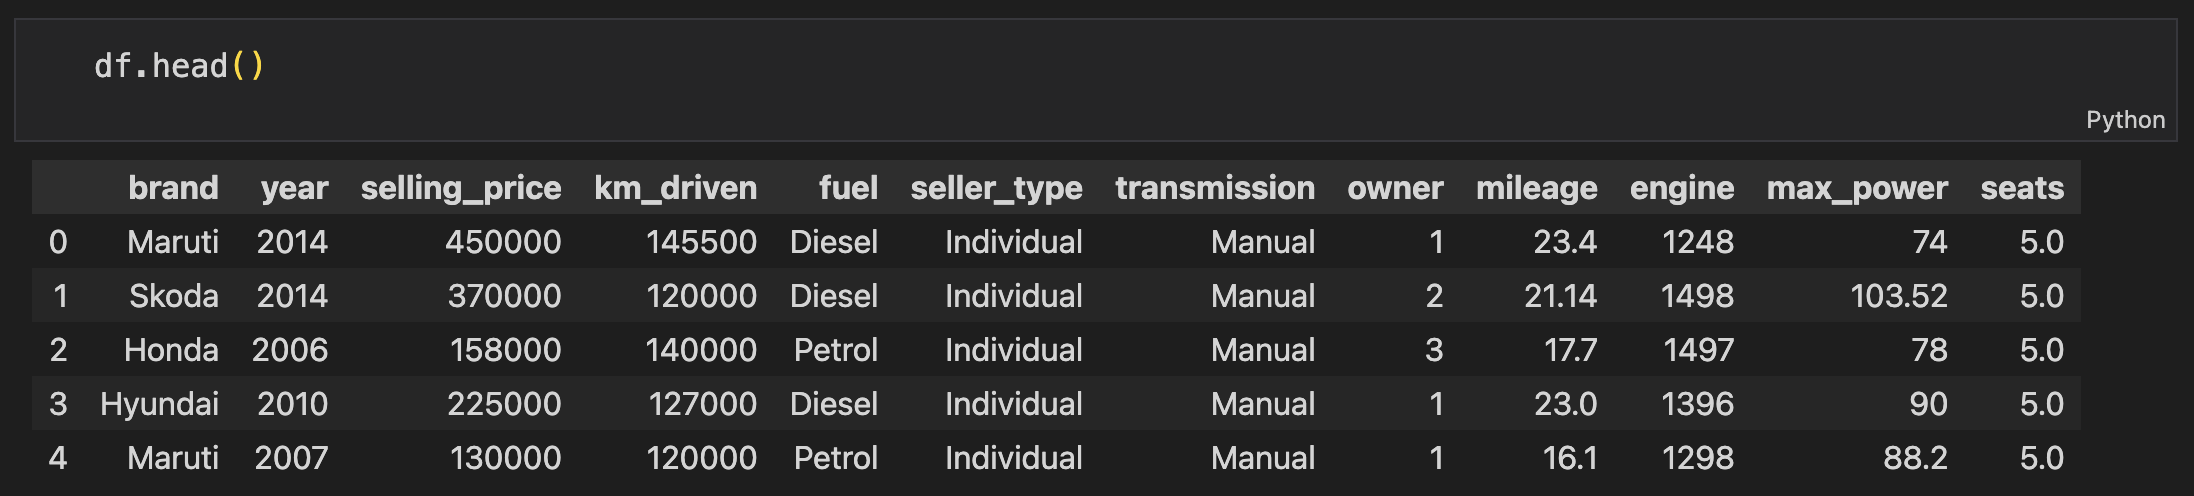
\includegraphics[width=0.9\textwidth]{media/fig1.png}
    \caption{Example of cleaned data}
\end{figure}

\task \textbf{Report} - In the end of the notebook, please write a 2-3 paragraphs summary deeply discussing and analysing the results.  Possible points of discussion:

\begin{itemize}
    \item Which features are important?  Which are not?  Why?
    \item Which algorithm performs well?  Which does not?  Why?  (here, you haven't learned about any algorithms yet, but you can search online a bit and start building an intuition)
\end{itemize}

\task \textbf{Deployment} - Develop a web-based application that contains the model.  Here you will be tasked to self-study how to deploy the model into production.  Here are some guidelines:

Here you have multiple options. Those who are veteran web developer may prefer their own web app stack which is welcomed. For those who are new to this realm, you may consider a simpler/one-stop solution rather than learning the traditional/flexible approach.

The goal of this task is to expose/deploy our model for public use via the web interface. The main scenario is the following:

\begin{enumerate}
    \item Users enter the domain on their browser. They land on your page.
    \item (optional) Users may need to navigate to a prediction page.
    \item Users read the instruction given on the page that instructs them on how the prediction works.
    \item Users find the input form, put in the appropriate data, and click submit. Note that when you receive the inputs from users, be reminded to scale your features before inputting into the model.  This scaler should be the same one that you use to scale your training features.
    \item Note that if users do not have information on certain field, you have to allow users to skip that field.  In that case, we recommend you to fill the missing field with imputation technique you have learned in the class.
    \item A moment later (depending on your model and hardware performance), the result is returned and printed below the form.
\end{enumerate}

Deploying aside, the app should work on the local environment (your machine) first.
I would suggest you use `Dash' by `Plotly' \url{https://dash.plotly.com/} as a one-stop solution.
Spend time studying the `Quick Start' tutorial on the site and also `Dash Fundamental'.
They are essential for you to know how `Dash' works.

The deliverable for the app would be, in GitHub, you have a folder `app' with `.Dockerfile', `docker-compose.yaml' files, and `code' folder.

\textbf{Bootstrap:} I know Dockerizing the app could be difficult for newcomers, you will get confused when searching for stuff online, especially, when you just trust ChatGPT to give you the right answer.
So, for those who want to postpone the process of learning ``Docker", here is the Dockerized Dash project \href{https://github.com/chaklam-silpasuwanchai/Machine-Learning/tree/main/Appendix/Appendix\%20-\%20Dash\%20Plotly}{link}. Don't worry, you will eventually need to do this yourself in this shortcoming weeks. You can not escape this.


\vspace{0.01\textheight}


\begin{center}
    Good luck :-)
\end{center}

\end{document}